\subsection{Overview: high-level components and interactions}
This section presents the overall system architecture by providing a high-level description of its components and the interaction between them. It outlines the architectural layers that composes the system and explains how they cooperate to deliver the required functionalities. Moreover, it discusses the key modeling and design choices adopted to satisfy the functional and non-functional requirements specified in the RASD document. \\[5pt]
The system’s architecture has been structured according to a four-tier model, a widely recognized design pattern that organizes the application into separate layers, each responsible for specific functions. This layered approach improves modularity, maintainability, scalability and fault tolerance, allowing each component to evolve independently without impacting the others.
The four tiers composing the architecture are the following:
\begin{itemize}
    \item \textbf{Presentation Tier:} Defines the user interface through which clients interact with the platform.
    \item \textbf{Web Server Tier:} Hosts the web server and manages incoming requests, routing them to the appropriate services.
    \item \textbf{Application Tier:} Contains the core business logic and processes application data. Application Tier is designed according to a microservices-based architectural approach.
    \item \textbf{Data Tier:} Handles data storage, management, and access through databases.
\end{itemize}
\begin{figure}[H]
\centering
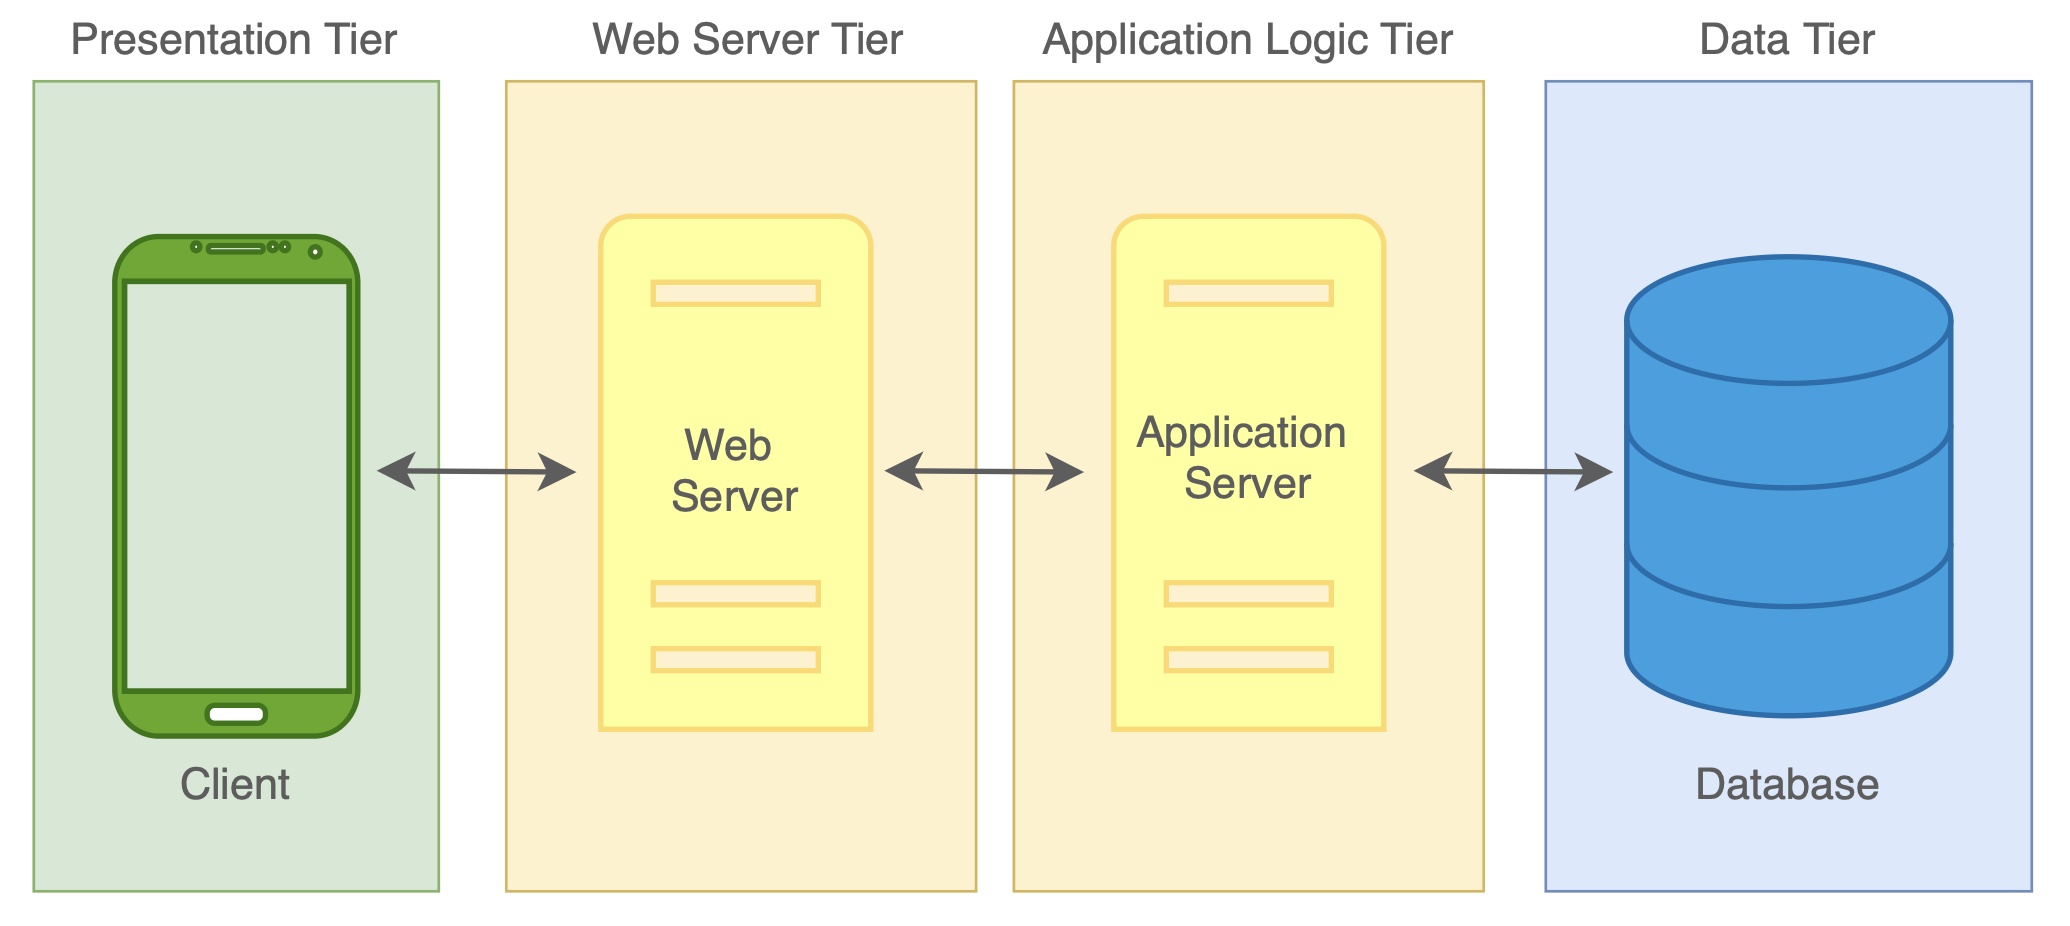
\includegraphics[width=0.8\textwidth]{Images/High Level View.png}
\caption{\label{fig:metamodel2}High level components diagram}
\end{figure}
\noindent{In particular, the Application Tier is designed according to a microservices-based architectural approach, where system functionalities are decomposed into independent and loosely coupled services. 
Although, for simplicity, the Application Tier and the Data Tier are represented in an abstract version as single components in the high-level architecture, in the actual implementation each microservice manages its own dedicated data store, in accordance with the database-per-service pattern. The internal structure and interactions of the individual services are described in detail in the following sections.}
\subsection{Component view}
The platform consists of several components grouped into two main categories: backend and frontend components. Notice that the backend comprehends Web Server and Application Logic tiers and it is organized according to a microservices architecture. Moreover, each component of the software is responsible for providing a specific service and implements one or more system functionalities.\\[8pt]
\textbf{Backend components}
\begin{itemize}
    \item \textit{Authentication service}
    \\ This service lets the users to perform sign up and login in the application. If a new user sign up, the service checks the email does not exist in the system or if an user is logging the system checks that the credentials are corrects.
    \item \textit{Account service}
    \\ This service stores and updates the cyclist profile information. It permits the cyclist edit his username, email, password and photos.
    \item \textit{Inventory service}
    \\ This service saved and shows cyclist's personal routes and paths. It supports filters by date, distance and score . When the cyclist open a path it returns the list of all the routes of that path and details
    \item \textit{ManagePath service}
    \\This service manages paths in the BPP . It creates automatically a new path when it is created a route on a non existing path. It manages the visibility of the path (public or private) and eventually the deletion of the path.
    \item \textit{ManageRoute service}
    \\This service manages routes, a single ride on a path. It lets user create a route either in manual mode or automatic mode. It also enriches the route with other detail and supports the operation of publish, unpublish and delete.
    \item \textit{Navigation system} 
    \\ this service implements a navigation support for the cyclist. When a cyclist selects a path the navigation system guides the cyclist along the streets of that path until the end point is reached.
    \item \textit{Recommendation system} 
    \\ This service supports the user search of a path. From a start and an end point received in input it recommends a list of path ranked by score. Moreover, the service merges different information from several routes on the same path keeping the path status updated.
    \item \textit{ManageSensorsData service}
    \\This service collects data from the mobile sensors (GPS,accelerometer,gyroscope) during the ride of the cyclist. It enriches the route with these information.
    \item \textit{API Gateway}
\\ This is the entry point for each app request. It forwards each request to the right microservices.    
    \item \textit{DBMSs}
    \\Each microservice owns its own database to store its data, keeping the services independent.
\end{itemize}
\textbf{Frontend components}
\begin{itemize}
    \item \textit{User Interface}
    \\ It is the app interface for users. It allows accessing all the features of BPP for the Cyclist and a smaller portion of them for the Guest. 
\end{itemize}
\begin{figure}[H]
\centering
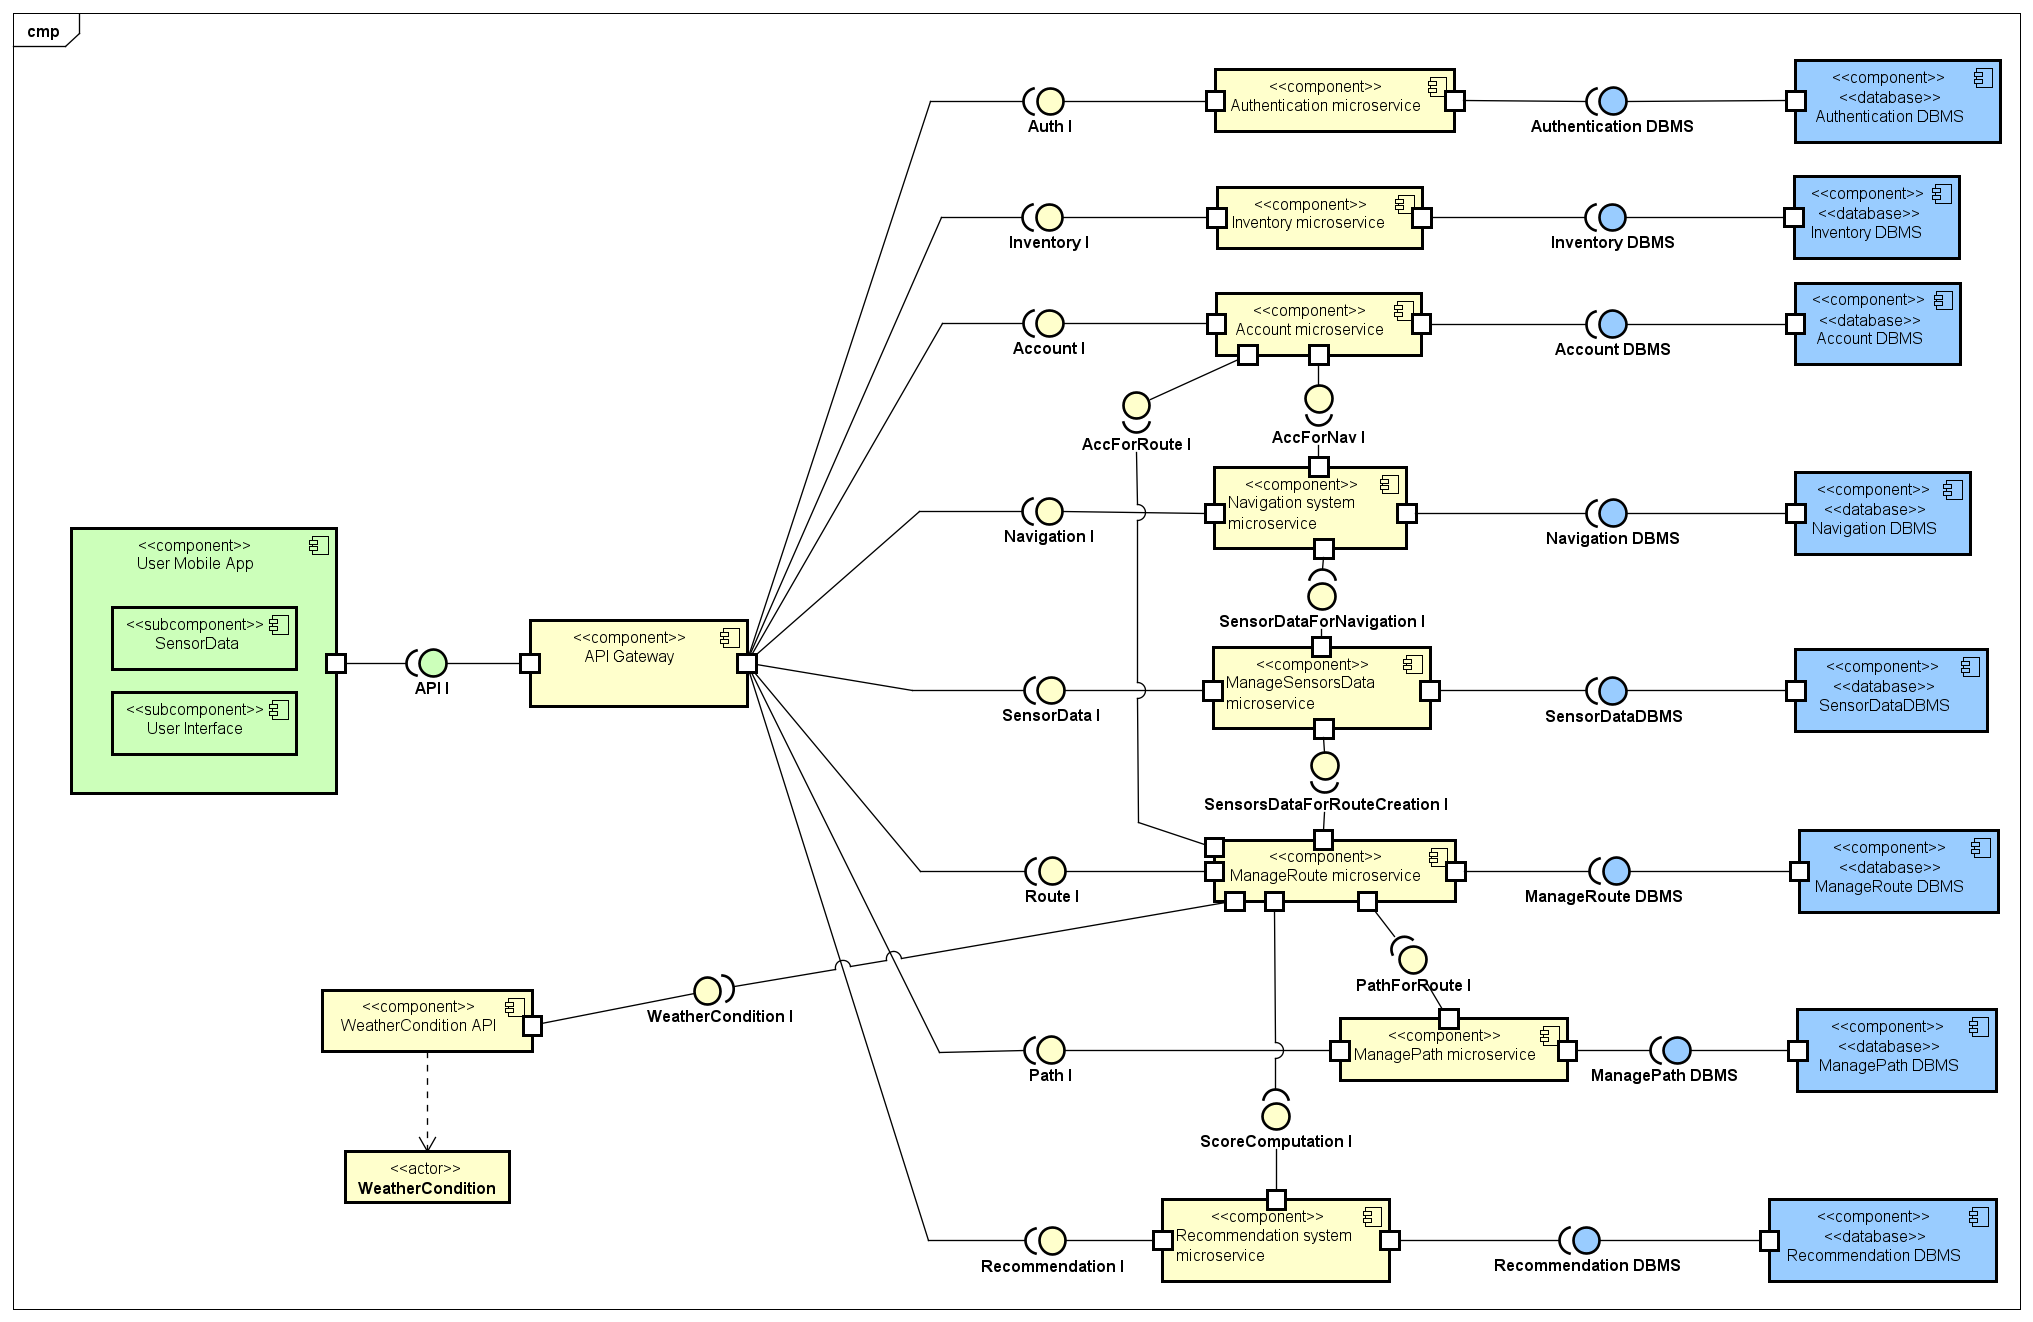
\includegraphics[width=\textwidth]{Images/Component Diagram.png}
\caption{\label{fig:metamodel2}Component diagram}
\end{figure}
\subsection{Deployment view}
Caching System \\
This component stores frequently used data in memory  making common requests faster . This also reduces load on the various services .
\subsection{Runtime view}
\subsection{Component interfaces}
\subsection{Selected Architectural Styles and Patterns}
\subsection{Other design decisions}